\begin{name}
	{\tenchude}
	{TOÁN 12}
	{LỚP TOÁN THẦY PHÁT}
	{Thời gian: 90 phút - Không kể thời gian phát đề}
\end{name}
\Opensolutionfile{ansbook}[ans/ansbookDe1]
\TN
\Opensolutionfile{ans}[ans/ansDe1-TN1]
\begin{ex}%[2D4N1-1]
Khẳng định nào sau đây là \textbf{sai}?
\choice
{ Mọi hàm số $f(x)$ liên tục trên đoạn $[a;b]$ đều có nguyên hàm trên đoạn $[a;b]$}
{\True $\displaystyle\int x^\alpha \mathrm{d}x=\dfrac{x^{\alpha +1}}{\alpha +1}+C$ ($C$ là hằng số, $\alpha $ là hằng số)}
{$\displaystyle\int \mathrm{e}^x\mathrm{d}x=\mathrm{e}^x+C$ ($C$ là hằng số)}
{$\displaystyle\int{\dfrac{1}{x}\mathrm{d}x=\ln \left| x \right|+C}$ ($C$ là hằng số) với $x\ne 0$}
\loigiai{
$\displaystyle\int x^{\alpha} \mathrm{d}\,x=\dfrac{x^{\alpha +1}}{\alpha +1}+C$ ($C$ là hằng số, $\alpha $ là hằng số và $\alpha \ne -1$).}
\end{ex}

\begin{ex}%[2D4N1-2]
Tìm họ nguyên hàm $F(x)$ của hàm số $f(x)=\dfrac{1}{x}$.
\choice
{\True  $F(x)=\ln \left| x \right|+C$}
{$F(x)=\ln x+C$}
{$F(x)=\ln \left| x \right|$}
{$F(x)=-\dfrac{1}{x^2}+C$}
\loigiai{
Áp dụng công thức nguyên hàm của hàm số ta có $\displaystyle\int{\frac{1}{x}\mathrm{d}\,x}=\ln \left| x \right|+C$.}
\end{ex}

\begin{ex}%[2D4N2-1]
Nếu $\displaystyle\int\limits_0^2f(x)\mathrm{\,d}x=5$ thì $\displaystyle\int\limits_0^2\left[2f(x)-1\right]\mathrm{\,d}x$ bằng
\choice
{\True $8$}
{$9$}
{$10$}
{$12$}
\loigiai{
Ta có $\displaystyle\int _0^2\left[2f(x)-1\right]\mathrm{\,d}x=2\displaystyle\int _0^2f(x)\mathrm{\,d}x-\displaystyle\int _0^21\mathrm{\,d}x=2\cdot 5-2=8$.}
\end{ex}

\begin{ex}%[2H5N1-1]
Trong không gian $Oxyz$, phương trình của mặt phẳng $(Oxy)$ là
\choice
{\True $z=0$}
{$x=0$}
{$y=0$}
{$x+y=0$}
\loigiai{
Phương trình của mặt phẳng $(Oxy)$ là $z=0$.
}
\end{ex}

\begin{ex}%[Mức độ 1]%[BG-12-New-4in1, Hiệp Hà]%[2H5N1-2]
Cho $(\alpha)$ vuông góc với giá của $\vec{a}=(-4;2;6)$. Vectơ nào dưới đây là một vectơ pháp tuyến của $(\alpha)$?
\choice
{$\vec{n_1}=(2;1;3)$}
{\True $\vec{n_2}=(-2;1;3)$}
{$\vec{n_3}=(4;-2;6)$}
{$\vec{n_4}=(4;2;-6)$}
\loigiai{
$(\alpha)$ vuông góc với giá của $\vec{a}=(-4;2;6)$ nên $\vec{a}$ là một vectơ pháp tuyến của $(\alpha)$.\\
Do đó $\vec{n_2}=\dfrac{1}{2}\vec{a}$ cũng là một vectơ pháp tuyến của $(\alpha)$.
}
\end{ex}

\begin{ex}%[2H5N2-1]
Trong không gian $Oxyz$, điểm nào dưới đây thuộc đường thẳng $d\colon\heva{& x=1+2t\\ & y=-3+t\\ & z=4+5t}$?
\choice
{$Q(4;1;3)$}
{$P(3;-2;-1)$}
{$N(2;1;5)$}
{\True $M(1;-3;4)$}
\loigiai{
Dễ thấy đường thẳng $d$ đi qua điểm $M(1;-3;4)$.
}
\end{ex}

\begin{ex}%[2025-TLOT-2018,Trần Xuân Hòa]%[2H5N2-2]
Trong không gian $O x y z$, vectơ nào sau đây là một vectơ chỉ phương của đường thẳng $\Delta\colon \dfrac{x-5}{8}=\dfrac{y-9}{6}=\dfrac{z-12}{3}$?
\choice
{\True $\overrightarrow{u}_1=(8 ; 6 ; 3)$}
{$\overrightarrow{u}_2=(8 ; 6 ;-3)$}
{$\overrightarrow{u}_3=(-8 ; 6 ;-3)$}
{$\overrightarrow{u}_4=(5 ; 9 ; 12)$}
\loigiai{
Vectơ chỉ phương của đường thẳng $\Delta\colon \dfrac{x-5}{8}=\dfrac{y-9}{6}=\dfrac{z-12}{3}$ là $\overrightarrow{u}_1=(8 ; 6 ; 3)$.
}
\end{ex}

\begin{ex}%[2H5N3-2]
Trong không gian $Oxyz$, mặt cầu $(S) \colon x^2+y^2+z^2+4x-2y+8z-1=0$ có tọa độ tâm là
\choice
{$(4;-2;8)$}
{ $(2;-1;4)$}
{\True $(-2;1;-4)$}
{$(2;-1;-4)$}
\loigiai{

}
\end{ex}

\begin{ex}%[2D6N1-1]
Cho $P(A)$, $P(B)>0$. Chọn khẳng định đúng trong các khẳng định sau.
\choice
{$\mathrm{P}(A\mid B)=\dfrac{\mathrm{P}(A\cup B)}{\mathrm{P}(A)}$}
{$\mathrm{P}(A\mid B)=\dfrac{\mathrm{P}(A\cup B)}{\mathrm{P}(B)}$}
{\True $\mathrm{P}(A\mid B)=\dfrac{\mathrm{P}(A\cap B)}{\mathrm{P}(B)}$}
{$\mathrm{P}(A\mid B)=\dfrac{\mathrm{P}(A\cap B)}{\mathrm{P}(A)}$}
\loigiai{
Nếu $\mathrm{P}(B)>0$ thì $\mathrm{P}(A\mid B)=\dfrac{\mathrm{P}(A\cap B)}{\mathrm{P}(B)}$.
}
\end{ex}

\begin{ex}%[2D6N2-1]
Cho hai biến cố ngẫu nhiên $A$, $B$ thoả mãn $\mathrm{P}(A)>0$ và $0<\mathrm{P}(B)<1$. Chọn khẳng định đúng trong các khẳng định sau.
\choice
{$\mathrm{P}(B\mid A)=\dfrac{\mathrm{P}(A)\cdot \mathrm{P}(A\mid \overline{B})}{\mathrm{P}(B)\cdot \mathrm{P}(A\mid B)+\mathrm{P}(B)\cdot \mathrm{P}(A\mid B)}$}
{$\mathrm{P}(B\mid A)=\dfrac{\mathrm{P}(\overline{B})\cdot \mathrm{P}(A\mid \overline{B})}{\mathrm{P}(B)\cdot \mathrm{P}(A\mid B)+\mathrm{P}(B)\cdot \mathrm{P}(A\mid B)}$}
{$\mathrm{P}(B\mid A)=\dfrac{\mathrm{P}(A)\cdot \mathrm{P}(A\mid B)}{\mathrm{P}(B)\cdot \mathrm{P}(A\mid B)+\mathrm{P}(\overline{B})\cdot \mathrm{P}(A\mid \overline{B})}$}
{\True $\mathrm{P}(B\mid A)=\dfrac{\mathrm{P}(B)\cdot \mathrm{P}(A\mid B)}{\mathrm{P}(B)\cdot \mathrm{P}(A\mid B)+\mathrm{P}(\overline{B})\cdot \mathrm{P}(A\mid \overline{B})}$}
\loigiai{
$\mathrm{P}(B\mid A)=\dfrac{\mathrm{P}(B)\cdot \mathrm{P}(A\mid B)}{\mathrm{P}(B)\cdot \mathrm{P}(A\mid B)+\mathrm{P}(\overline{B})\cdot \mathrm{P}(A\mid \overline{B})}$.
}
\end{ex}

\begin{ex}%[2D6N2-3]
Cho hai biến cố $A$, $B$ thoả mãn $\mathrm{P}(A)=0{,}4$; $\mathrm{P}(B)=0{,}3$; $\mathrm{P}(A | B)=0{,}25$. Khi đó, $\mathrm{P}(B | A)$ bằng:
\choice
{\True $0{,}1875$}
{$0{,}48$}
{$0{,}333$}
{$0{,}95$}
\loigiai{
Theo công thức Bayes, ta có $\mathrm{P}(B|A)=\dfrac{\mathrm{P}(B) \cdot \mathrm{P}(A|B)}{\mathrm{P}(A)}=\dfrac{0{,}3 \cdot 0{,}25}{0{,}4}=0{,}1875$.
}
\end{ex}

\begin{ex}%[2H5N3-3]
Trong không gian $Oxyz$, mặt cầu có tâm $I(2; 1; -3)$ và bán kính $9$ và có phương trình là
\choice
{\True $(x-2)^2+(y-1)^2+(z+3)^2=81$}
{$(x+2)^2+(y+1)^2+(z-3)^2=81$}
{$(x-2)^2+(y-1)^2+(z+3)^2=9$}
{$(x+2)^2+(y+1)^2+(z-3)^2=9$}
\loigiai{
Trong không gian $Oxyz$, mặt cầu có tâm $I(2; 1; -3)$ và bán kính $9$ và có phương trình là $(x-2)^2+(y-1)^2+(z+3)^2=81$.
}
\end{ex}
\Closesolutionfile{ans}

\TNTF
\Opensolutionfile{ans}[ans/ansDe1-TN2]
\begin{ex}
Cho hàm số $f(x)=\dfrac{2x+1}{x+2}$.
\choiceTF
{\True $\displaystyle\int f'(x)\mathrm{\,d}x=\dfrac{2x+1}{x+2}+C$}
{$\displaystyle\int f(x)\mathrm{\,d}x=2\ln \left| x+2 \right|+C$}
{\True $\displaystyle\int_{-1}^2 [f'(x)-2] \mathrm{\,d}x >-3$}
{\True Diện tích hình phẳng giới hạn với đường cong $y=f(x)$, trục hoành và các đường thẳng $x=-1$ và $x=2$ bằng $4+6\ln a$ và $0<a<1$}
\loigiai{
    \begin{itemchoice}
    \itemch $\displaystyle\int f'(x)\mathrm{\,d}x= f(x)+C = \dfrac{2x+1}{x+2}+C$.
    \itemch $\displaystyle\int f(x)\mathrm{\,d}x=\displaystyle\int \left(2-\dfrac{3}{x+2}\right)\mathrm{\,d}x=2x-3\ln \left| x+2 \right|+C$.
    \itemch $\displaystyle\int_{-1}^2 [f'(x)-2] \mathrm{\,d}x=f(2)-f(-1)-2x\vert_{-1}^2=\dfrac54+\dfrac13-2\cdots 3=0{,}5>-3$.
    \itemch Diện tích hình phẳng giới hạn với đường cong $y=f(x)$, trục hoành và các đường thẳng $x=-1$ và $x=2$ là 
    $$S=\displaystyle\int_{-1}^2 |f(x)| \mathrm{\,d}x = -\int_{-1}^{-\frac12} f(x) \mathrm{\,d}x + \int_{-\frac12}^{2} f(x) \mathrm{\,d}x = - \left(2x-3\ln \left| x+2 \right| \right)\vert_{-1}^{-\frac12} + \left(2x-3\ln \left| x+2 \right| \right)\vert_{-\frac12}^{2} = 4+3\ln \dfrac{9}{16} = 4+6\ln \dfrac{3}{4}$$
    Vậy $0<a=\dfrac{3}{4}<1$.
    \end{itemchoice}
}


\end{ex}

\begin{ex}%[Mức độ 2]%[BG-12-New-4in1, Hiệp Hà]%[2H5H1-2]
Cho mặt phẳng $(\alpha)$ đi qua $A(-1;1;2)$ có cặp vectơ chỉ phương là $\vec{a} = (1; -2; 3)$ và $\vec{b}= (2; 1; -1)$.
\choiceTF
{$\vec{a}$ có giá song song với mặt phẳng $(\alpha)$}
{\True Mặt phẳng $(\alpha)$ có phương trình là $x-7y-5z+18=0$}
{Đường thẳng $d \colon \dfrac{x+1}{2}=\dfrac{y-1}{1}=\dfrac{z-2}{-1}$ song song với mặt phẳng $(\alpha)$}
{Mặt phẳng $(\alpha)$ cắt mặt cầu $(S)$ có tâm $I(2; 1; -3)$ và bán kính $1$ theo giao tuyến là một đường tròn}
\loigiai{
\begin{itemchoice}
\itemch $\vec{a}$ là một vectơ trong cặp vectơ chỉ phương nên $\vec{a}$ có giá song song hoặc nằm trong mặt phẳng $(\alpha)$.
\itemch Ta có
\[
\begin{aligned}
\vec{n}=[\vec{a}, \vec{b}] & =\left(\left|\begin{array}{cc}
-2 & 3 \\ 1 & -1
\end{array}\right| ;\left|\begin{array}{cc}
3 & 1 \\ -1 & 2
\end{array}\right| ;\left|\begin{array}{cc}
1 & -2 \\ 2 & 1
\end{array}\right|\right) \\
& =(-1; 7; 5) .
\end{aligned}
\]
Do đó $\vec{n_1}=(1;-7;-5) =-\vec{n}$ là một vectơ pháp tuyến của mặt phẳng $(\alpha)$ nên mặt phẳng $(\alpha)$ đi qua $A(-1;1;2)$ có phương trình là
$$1(x+1)-7(y-1)-5(z-2)=0 \Leftrightarrow x-7y-5z+18=0.$$
\itemch Đường thẳng $d \colon \dfrac{x+1}{2}=\dfrac{y-1}{1}=\dfrac{z-2}{-1}$ có vectơ chỉ phương là $\vec{b}=(2;1;-1)$ và đi qua $A(-1;1;2)$ nên $d$ nằm trên $(\alpha)$.
\itemch Vì $d(I,(\alpha))=\dfrac{\left| 1\cdot 2-7\cdot 1-5\cdot (-3) \right|}{\sqrt{1^2+7^2+5^2}} = \dfrac{2\sqrt{3}}{3}>1$ nên mặt phẳng $(\alpha)$ không cắt mặt cầu $(S)$.
\end{itemchoice}
}
\end{ex}
\Closesolutionfile{ans}

\TNSA
\Opensolutionfile{ans}[ans/ansDe1-TN3]
\begin{ex}%[2D4H1-4]
Cho hàm số $f(x)=2x+\mathrm{e}^x$. Một nguyên hàm $F(x)$ của hàm số $f(x)$ thỏa mãn $F(0)=2024$. Biết $F(x)=ax^2+b\mathrm{e}^x+c$, giá trị của $a+b+c$ là
\shortans{$2025$}
\loigiai{
Ta có $\displaystyle\int f(x)\mathrm{\,d}x=\displaystyle\int (2x+\mathrm{e}^x)\mathrm{\,d}x=x^2+\mathrm{e}^x+C$.\\
Có $F(x)$ là một nguyên hàm của $f(x)$ và $F(0)=2024$.\\
Tìm được $\heva{&F(x)=x^2+\mathrm{e}^x+C\\ &F(0)=2024} \Rightarrow 1+C=2024 \Leftrightarrow C=2023$.\\
Suy ra $F(x)=x^2+\mathrm{e}^x+2023$.\\
Vậy $a+b+c=2025$.
}
\end{ex}

\begin{ex}%[2D4V2-6]
Gọi $h(t)$ cm là mức nước trong bồn chứa sau khi bơm được $t$ giây. Biết rằng tốc độ tăng giảm của mực nước là $h^{\prime}(t)=\dfrac{1}{5} \sqrt[3]{t+8}$ (cm/s) và lúc đầu bồn không có nước. Tìm mức nước ở bồn (đơn vị: cm) sau khi bơm nước được $6$ giây (làm tròn đến chữ số hàng phần trăm).
\shortans{$2{,}66$}
\loigiai{Hàm $h(t)=\displaystyle\int\limits \dfrac{1}{5} \sqrt[3]{t+8} \mathrm{\,d} t=\dfrac{3}{20}(t+8) \sqrt[3]{t+8}+C$.\\
Lúc $t=0$, bồn không chứa nước. Suy ra $h(0)=0 \Rightarrow \dfrac{12}{5}+C=0 \Leftrightarrow C=-\dfrac{12}{5}$.\\
Vậy, hàm $h(t)=\dfrac{3}{20}(t+8) \sqrt[3]{t+8}-\dfrac{12}{5}$.\\
Mức nước trong bồn sau $6$ giây là $h(6) \simeq 2{,}66$ cm.
}
\end{ex}

\begin{ex}%[2H5V2-8]
    Hình vẽ dưới đây là hình ảnh Cầu Cổng Vàng (The Golden Gate Bridge) ở Mỹ. Xét hệ trục toạ độ $O x y z$ với $O$ là bệ của chân cột trụ tại mặt nước, trục $O z$ trùng với cột trụ, mặt phẳng $O x y$ là mặt nước và xem như trục $O y$ cùng phương với cầu như hình vẽ. Dây cáp $A D$ (xem như là một đoạn thẳng) đi qua đỉnh $D$ thuộc trục $O z$ và điểm $A$ thuộc mặt phẳng $O y z$, trong đó điểm $D$ là đỉnh cột trụ cách mặt nước $227$ m, điểm $A$ cách mặt nước $75$ m và cách trục $O z$ khoảng $343$ m. \begin{flushright}
    \textit{(Nguồn: https://www.goldengate.org/assets/1/6/ggb-exhibit-chapter-statistics.pdf)}
    \end{flushright}
    \begin{center}
    \includegraphics[scale=.5]{images/Cau-cong-vang}
    \end{center}
    Giả sử ta dùng một đoạn dây nối điểm $N$ trên dây cáp $A D$ và điểm $M$ trên thành cầu, biết $M$ cách mặt nước $75$ m và $M N$ song song với cột trụ. Tính độ dài $M N$ (đơn vị mét) biết điểm $M$ cách trục $O z$ một khoảng bằng $230$ m (kết quả làm tròn đến hàng phần mười).
    \shortans{$50{,}1$}
    \loigiai{
    Chọn một đơn vị trên các trục bằng $1$ m.\\
    Ta có $D(0 ; 0 ; 227),$ $ A(0 ;-343 ; 75),$ $ M(0 ;-230 ; 75)$, $\overrightarrow{A D}=(0 ; 343 ; 152)$.\\ Phương trình đường thẳng $A D\colon \heva{&x=0 \\& y=343 t \\& z=227+152 t} \Rightarrow N(0 ; 343 t ; 227+152 t)$.\\
    Ta có $\overrightarrow{M N}=(0 ; 343 t+230 ; 152+152 t)$, $M N$ song song với trục $O z$, suy ra \[ 343 t+230=0 \Rightarrow t=-\dfrac{230}{343} \Rightarrow M N=152+152 \cdot \left(-\dfrac{230}{343}\right) \approx 50,1(m).\]
    }
    \end{ex}

\begin{ex}%[2D6V1-3]
Ông An hằng ngày đi làm bằng xe máy hoặc xe buýt. Nếu hôm nay ông đi làm bằng xe buýt thì xác suất để hôm sau ông đi làm bằng xe máy là $0,4$ . Nếu hôm nay ông đi làm bằng xe máy thì xác suất để hôm sau ông đi làm bằng xe buýt là $0,7$ . Xét một tuần mà thứ Hai ông An đi làm bằng xe buýt. Tính xác suất để thứ Tư trong tuần ông An đi làm bằng xe máy.

\shortans{0,36}
\loigiai
{
Gọi $A$ là biến cố \textquotedblleft Thứ Ba, ông An đi làm bằng xe máy\textquotedblright.\\
$B$ là biến cố \textquotedblleft Thứ Tư, ông An đi làm bằng xe máy\textquotedblright.\\
Khi đó $\heva{&P(A) = 0{,}4&\Rightarrow& P(\overline{A}) = 1-0{,}4 = 0{,}6\\ &P(\overline{B}|A) = 0{,}7 &\Rightarrow& P(B|A) = 1-0{,}7 = 0{,}3\\ &P(B|\overline{A}) = 0{,}4 &\Rightarrow& P(\overline{B}|\overline{A}) = 1-0{,}4=0{,}6.}$
\begin{center}
\begin{tikzpicture}[>=stealth]
%Khung 1
\draw (1,3.0) node{\textbf{Thứ Hai}};
\draw (-0,-1) rectangle (2.2,0);
\draw (1.1,-0.5) node{Buýt};
%Mui ten 1,2
\draw [->] (2.2,-0.5)--(3.8,1.6) node[pos=0.5,sloped,above]{$0{,}4$};
\draw [->] (2.2,-0.5)--(3.8,-2.6) node[pos=0.5,sloped,below]{\color{red}$0{,}6$};
%Khung 2.1
\draw (4.5,3.0) node{\textbf{Thứ Ba}};
\draw (3.8,1.1) rectangle (5.1,2.1);
\draw (8.9/2,1.6) node{$A$} ;
%Khung 2.2
\draw (3.8,-2.1) rectangle (5.1,-3.1);
\draw (8.9/2,-2.6) node{$\overline{A}$};
%Mui ten 3,4
\draw [->] (5.1,1.6)--(6.5,2.6) node[pos=0.5,sloped,above]{\color{red}$0{,}3$};
\draw [->] (5.1,1.6)--(6.5,0.6) node[pos=0.5,sloped,below]{$0{,}7$};
%Mui ten 5,6
\draw [->] (5.1,-2.6)--(6.5,-1.6) node[pos=0.5,sloped,above]{$0{,}4$};
\draw [->] (5.1,-2.6)--(6.5,-3.6) node[pos=0.5,sloped,below]{\color{red}$0{,}6$};
%Khung 3.1
\draw (6.5,2.2) rectangle (7.7,3.2);
\draw (7.1,5.4/2) node{$B$} ;
%Khung 3.2
\draw (7.0,3.7) node{\textbf{Thứ Tư}};
\draw (6.5,1.2) rectangle (7.7,0.2);
\draw (7.1,1.4/2) node{$\overline{B}$} ;
%Khung 3.3
\draw (6.5,-1.1) rectangle (7.7,-2.1);
\draw (7.1,-3.2/2) node{$B$} ;
%Khung 3.3
\draw (6.5,-2.9) rectangle (7.7,-3.9);
\draw (7.1,-3.4) node{$\overline{B}$} ;
%Kết quả
\draw (9.5,3.7) node{\textbf{Kết quả}};
\draw (9.5,2.7) node{$AB$};
\draw (9.5,0.7) node{$A \overline{B}$};
\draw (9.5,-1.6) node{$\overline{A}B$};
\draw (9.5,-3.4) node{$\overline{A}~\overline{B}$};
%Xác suất
\draw (12.5,3.7) node{\textbf{Xác suất}};
\draw (12.5,2.7) node{$0{,}12$};
\draw (12.5,0.7) node{$0{,}28$};
\draw (12.5,-1.6) node{$0{,}24$};
\draw (12.5,-3.4) node{$0{,}36$};
\end{tikzpicture}
\end{center}
Áp dụng công thức xác suất toàn phần để tính xác suất thứ Tư ông An đi làm bằng xe máy là
\[P(B) = P(A) \cdot P(B|A) + P(\overline{A}) \cdot P(B|\overline{A}) = 0{,}4 \cdot 0{,}3 + 0{,}6 \cdot 0{,}4 = 0{,}36.\]
}
\end{ex}
\TL
\begin{ex}%[2H5H2-3]%[Dự án 2025 - Đề cấu trúc mới của Bộ theo [Thành Đức Trung]
Trong không gian $Oxyz$, cho tam giác $ABC$ có $A(0;0;1)$, $B(-3;2;0)$, $C(2;-2;3)$. Viết phương trình đường cao kẻ từ $B$ của tam giác $ABC$.% đi qua điểm $K(a;b;-2)$. Tính $ab$.
% \shortans{$-2$}
\loigiai
{
Gọi $\Delta$ là đường cao kẻ từ $B$ của tam giác $ABC$.\\
Ta có $\heva{& \overrightarrow{AB}=(-3;2;-1) \\ & \overrightarrow{AC}=(2;-2;2)} \Rightarrow \left[\overrightarrow{AB},\overrightarrow{AC}\right]=(2;4;2)$. \\
Suy ra một véc-tơ pháp tuyến của mặt phẳng $(ABC)$ là $\overrightarrow{n}=(1;2;1)$.\\
Ta có $\heva{ & \Delta \subset(ABC) \\ & \Delta \perp AC}$, suy ra đường thẳng $\Delta$ nhận $\left[\overrightarrow{n},\overrightarrow{AC}\right]$ làm một véc-tơ chỉ phương.\\
Có $\left[\overrightarrow{n},\overrightarrow{AC}\right]=(6;0;-6)=6\overrightarrow{u}$ với $\overrightarrow{u}=(1;0;-1)$. \\
Suy ra đường thẳng $\Delta$ nhận $\overrightarrow{u}=(1;0;-1)$ làm véc-tơ chỉ phương.\\
Do đó phương trình đường thẳng $\Delta$ là $\Delta \colon \heva{ & x=-3+t \\ & y=2 \\ & z=-t} $%\Rightarrow K(-1;2;-2)$.\\
% Vậy $a=-1$; $b=2$ và $ab=-2$.
}
\end{ex}

\begin{ex}%[BAI-GIANG-12-4IN1, Võ Thị Thùy Trang]%[Cánh diều]%[2D6C2-4]
Giả sử có một loại bệnh mà tỉ lệ người mắc bệnh là $0{,}1\%$. Giả sử có một loại xét nghiệm, mà ai mắc bệnh khi xét nghiệm cũng có phản ứng dương tính, nhưng tỉ lệ phản ứng dương tính giả là $5\%$ (tức là trong số những người không bị bệnh có $5\%$ số người xét nghiệm lại có phản ứng dương tính). Khi một người xét nghiệm có phản ứng dương tính thì khả năng mắc bệnh của người đó là bao nhiêu phần trăm (làm tròn kết quả đến hàng phần trăm)?
% \shortans{$1{,}96$}
\loigiai{
\begin{itemize}
\item Xét hai biến cố\\
$K$ \lq\lq Người được chọn ra không mắc bệnh\rq\rq;\\
$D$ \lq\lq Người được chọn ra có phản ứng dương tính\rq\rq.\\
Do tỉ lệ người mắc bệnh là $0{,}1 \%=0{,}001$ nên $\mathrm{P}(K)=1-0{,}001=0{,}999$.\\
Trong số những người không mắc bệnh có $5 \%$ số người có phản ứng dương tính nên \break$\mathrm{P}(D \mid K)=5 \%=0{,}05$. Vì ai mắc bệnh khi xét nghiệm cũng có phản ứng dương tính nên $\mathrm{P}(D \mid \overline{K})=1$.\\
Sơ đồ hình cây ở bên dưới biểu thị tình huống đã cho.
\begin{center}
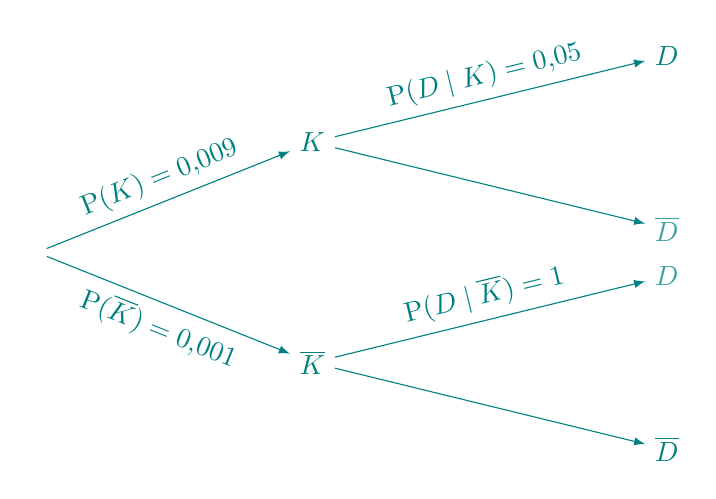
\begin{tikzpicture}[teal,grow=right, edge from parent/.style={draw,-latex}, label distance = 0.2cm,
level 1/.style = {level distance=3.5cm, sibling distance=28mm},
level 2/.style = {level distance=4.5cm, sibling distance=22mm},
level 3/.style = {level distance=4.5cm, sibling distance=22mm},
]

\node {}
child {node {$\overline{K}$
}
child {node {$\overline {D}$}
}
child {node[opacity=.75] {$D$}
edge from parent
node[above,sloped] {$\mathrm{P}(D\mid \overline {K})=1$}
}
edge from parent
node[below,sloped] {$\mathrm{P}(\overline {K})=0{,}001$}
}
child {node[] {$K$}
child {node[opacity=.75] {$\overline {D}$}
}
child {node[] {$D$}
edge from parent
node[above,sloped] {$\mathrm{P}(D\mid K)=0{,}05$}
}
edge from parent
node[above,sloped] {$\mathrm{P}(K)=0{,}009$}
};
\end{tikzpicture}
\end{center}
\item Ta thấy, khả năng mắc bệnh của một người xét nghiệm có phản ứng dương tính chính là $\mathrm{P}(\overline{K} \mid D)$. Áp dụng công thức Bayes, ta có
\[
\mathrm{P}(\overline{K}|D)=\dfrac{\mathrm{P}(\overline{K}) \cdot \mathrm{P}(D| \overline{K})}{\mathrm{P}(\overline{K}) \cdot \mathrm{P}(D| \overline{K})+\mathrm{P}(K) \cdot \mathrm{P}(D| K)}=\dfrac{0{,}001}{0{,}001+0{,}999 \cdot 0{,}05} \approx 1{,}96 \% .
\]
Vậy xác suất mắc bệnh của một người xét nghiệm có phản ứng dương tính là $1{,}96\%$.
\end{itemize}
}
\end{ex}

\begin{ex}%[Mức độ 3]giảng 12 New - 4in1, Đoàn Hùng]%[2H5C1-7]
Trong không gian với hệ tọa độ $Oxyz$, cho ba điểm $A(1;4;5)$, $B(3;4;0)$, $C(2;-1;0)$ và mặt phẳng $(P)\colon 3x-3y-2z-12=0$. Gọi $M(a;b;c)$ thuộc $(P)$ sao cho $MA^2+MB^2+3MC^2$ đạt giá trị nhỏ nhất. Tính tổng $a+b+c$.
% \shortans{$3$}
\loigiai{
Gọi $I(x;y;z)$ là điểm thỏa mãn $\overrightarrow{IA}+\overrightarrow{IB}+3\overrightarrow{IC}=\overrightarrow{0}$.\\
Ta có $\overrightarrow{IA}=(1-x;4-y;5-z)$, $\overrightarrow{IB}=(3-x;4-y;-z)$ và $3\overrightarrow{IC}=(6-3x;-3-3y;-3z)$.\\
Từ ta có hệ phương trình: $\heva{&1-x+3-x+6-3x=0\\&4-y+4-y-3-3y=0\\&5-z-z-3z=0} \Leftrightarrow \heva{&x=2\\&y=1\\&z=1} $$\Rightarrow I(2;1;1)$.\\
Ta có
\begin{itemize}
\item $MA^2=\overrightarrow{MA}^2=(\overrightarrow{MI}+\overrightarrow{IA})^2=MI^2+2\overrightarrow{MI}\cdot \overrightarrow{IA}+IA^2$.
\item $MB^2=\overrightarrow{MB}^2=(\overrightarrow{MI}+\overrightarrow{IB})^2=MI^2+2\overrightarrow{MI}\cdot \overrightarrow{IB}+IB^2$.
\item $3MC^2=3\overrightarrow{MC}^2=3(\overrightarrow{MI}+\overrightarrow{IC})^2=3(MI^2+2\overrightarrow{MI}\cdot \overrightarrow{IC}+IC^2)$.
\end{itemize}
Do đó $S=MA^2+MB^2+3MC^2=5MI^2+IA^2+IB^2+3IC^2$.\\
Do $IA^2+IB^2+3IC^2$ không đổi nên $S$ đạt giá trị nhỏ nhất khi và chỉ khi $MI$ đạt giá trị nhỏ nhất. Tức là $M$ là hình chiếu của $I$ lên mặt phẳng $(P)\colon 3x-3y-2z-12=0$ Suy ra $\overrightarrow{IM}$ cùng phương với véc-tơ chỉ phương pháp tuyến $\overrightarrow{n}=(3;-3;-2)$ của $(P)$.\\
Suy ra $M(2+3t;1-3t;1-2t)$.\\
Vì $M\in (P)$ nên $3(2+3t)-3(1-3t)-2(1-2t)-12=0\Leftrightarrow 22t-11=0\Leftrightarrow t=\dfrac{1}{2}$.\\
Suy ra $M\left(\dfrac{7}{2};-\dfrac{1}{2};0\right)$.\\
Vậy $a+b+c=\dfrac{7}{2}-\dfrac{1}{2}=3$.
}
\end{ex}
\Closesolutionfile{ans}


\Closesolutionfile{ansbook}
